\chapter{Implementation}


\section{WebExtensions}
\paragraph{Write a blah blah paragraph, can be short, about the basic structure of WebExtension. The following are Manifest Keys that will be required for my implementation.}

\begin{enumerate}
\item \emph{manifest\_version}: Always 2
\item \emph{name}: Name of the implementation
\item \emph{description}: Description of the extension
\item \emph{version}: The version of the software
\item \emph{author}: The name of the developer
\item \emph{applications}: Also known as the \emph{brower\_specific\_settings} contains keys that are specific to the particular host application. 
\begin{center}
\begin{minted}{javascript}
"background": {
    "page": "background.html"
},
\end{minted}
\end{center}
\end{enumerate}


\paragraph{In Thunderbird, all WebExtension API can be accessed through the browser.* namespace, as with Firefox, but also through the messenger.* namespace, which is a better fit for Thunderbird.}\footnote{From website: https://developer.thunderbird.net/add-ons/mailextensions/hello-world-add-on/using-webextension-apis}

\paragraph{messenger.tabs.query}
\subparagraph{The tabs API provides access to Thunderbird's tabs. In some cases, since the call is executed from where it is called from, it may be necessary to execute tabs \emph{message\_display\_action} and not from inside the tab we are looking for.}

\paragraph{messenger.messageDisplay.getDisplayedMessage()}
\subparagraph{the \emph{getDisplayedMessage} method of the \emph{messageDisplay API} provides access to the currently viewed message in a given tab. It returns a promise for a \emph{MessageHeader} object from the \emph{message API} with basic imformation about the message.}\footnote{The getDisplayMessage method requires the messageRead permission, which needs to be added ot the permissions key of the manifest.json file.}

\paragraph{messenger.messages.getFull()}
\subparagraph{The \emph{getFull()} method returns a Promise for a MessagePart object, which relates to messages containing multiple MIME parts. The headers member of the part returned by getFull includes the headers of the message.}

\paragraph{Steps to create an addon in Thunderbird.}

\subsection{Using a background page}
% Adding the following, may or may not use, but learning them can't hurt?
\paragraph{First, we need to add "backgrounds" to our manifest.}

\begin{center}
\begin{minted}{javascript}
"background": {
    "page": "background.html"
},
\end{minted}
\end{center}

\paragraph{Additionally, we'll need an html and javascript document, as well as keep the manifest updated.}

\begin{center}
\begin{minted}{html}
<!DOCTYPE html>
<html>
<head>
    <meta charset="utf-8"/>
    <script src="background.js" type="module"></script>
</head>
</html>
\end{minted}
\end{center}


\begin{enumerate}
\item Create manifest.json
\item Have it reference a folder (that it is outside of), like "MyAddon", which contains
\begin{itemize}
\item myaddon.html
\item myaddon.css
\item myaddon.js
\end{itemize}
\item Then, create another folder named "images", for images.
\item To install, open thunderbird
\item click on the hamburger button on the right side of tb
\item select "Debug Add-ons"
\item blick on "Load Temporary Add-on..." button
\item navigate to the previously created manifest.json file.
\end{enumerate}

\paragraph{The Add-on should be fully functional now.}


\section{Javascript Cryptography}

\paragraph{Originally, the researcher was not sure how best to implement cryptography within a Thunderbird add-on. Implementing my own javascript AES algorithm, while ideal, was not realistic--or adviceable--with the time constraints of this thesis. Thus, the issue would be finding an existing library or API that had done the javascript cryptographic implementations.}

\paragraph{For this task, there were three necessary conditions:}

\begin{itemize}
\item A clear, easily identifiable, and reputable source/owners
\item Existing, easily obtainable, and comprehensive documentation
\item Open source, easily available code
\end{itemize}

\paragraph{and, slightly less important, actively maintained.}

\paragraph{Meeting the above criteria was not as simple as it would seem. There were many options that met some of the conditions, but meeting them all was more challenging. Ultimately, however, the researcher was satisfied with the Stanford Javascript Crypto Library (SJCL) meeting the above full criteria.}\cite[Website]{SJCL}

\paragraph{The usage is pretty straight forward, and will work for this implementation. Simply linking the javascript source in the html file (See reference figure: \ref{fig: exampleSJCL_html}).:}

\begin{figure}[H]
\begin{minted}[breaklines]{html}
<!DOCTYPE html>
<html>
<head>
    <meta charset="utf-8"/>
    <script src="http://bitwiseshiftleft.github.io/sjcl/sjcl.js"></script>
</head>
</html>
\end{minted}
\caption{\label{fig: exampleSJCL_html} Example of linking SJCL in HTML}
\end{figure}

\paragraph{and, the javascript can simply be used as follows (See reference figure: \ref{fig: exampleSJCL_js}):}

\begin{figure}[H]
\centering
\begin{minted}[breaklines]{javascript}
var ciphertext = sjcl.encrypt("reallyHardPasswordNoOneCouldEveryGuess", "Hello World!");
var plaintext = sjcl.decrypt("reallyHardPasswordNoOneCouldEveryGuess", ciphertext);
console.log("plain text: " + plaintext);
console.log("cipher text: " + ciphertext);
console.log("plain text - again!: " + plaintext);
\end{minted}
\caption{\label{fig: exampleSJCL_js} Example of javascript SJCL}
\end{figure}

\paragraph{giving the following result (See reference figure: \ref{fig: exampleSJCL}):}

\begin{figure}[H]
\centering
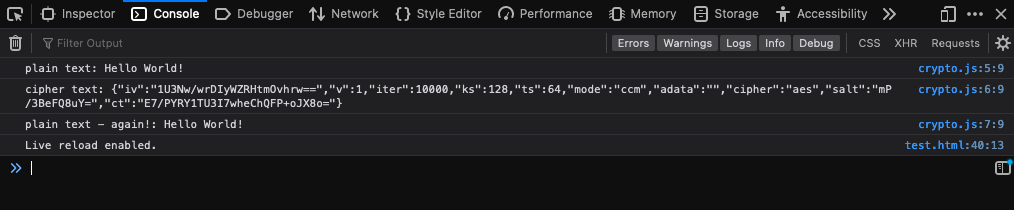
\includegraphics[width=0.9\textwidth]{exampleSJCL.png}
\caption{\label{fig: exampleSJCL} Example output to Firefox console}
\end{figure}

\paragraph{The usage is pretty straight forward, and will meet our needs.}

\section{Implementation Details}

